\sisetup{separate-uncertainty=true,detect-weight=true,detect-inline-weight=math}

\section{Experiments and Results}

% \uselengthunit{in}\printlength{\textwidth} = 4.8041 in
% \uselengthunit{mm}\printlength{\textwidth} = 121.99854 mm

%\subsection{Data Sets and Pre-processing}

We evaluated the proposed method on a large data set from a multi-center MS
clinical trial. The data set, acquired from 67 different scanning sites,
consists of 377 pairs of FLAIR and T1-weighted MRIs from 195 subjects with a
resolution of \num{256x256x60} voxels and a voxel size of
\SI{0.936x0.936x3.000}{\milli\metre}. All images were skull-stripped using the
brain extraction tool (BET) \cite{jenkinson2005bet2}, followed by an intensity
normalization to the interval $[0,1]$, and a 6 degrees-of-freedom intra-subject
registration. To speed-up the training, all images were cropped to a
\num{164x206x52} voxel region-of-interest with the brain roughly centered. We
used 300 image pairs for pre-training and fine-tuning, and the remaining 77
image pairs for evaluation. Pre-training and fine-tuning were performed using a
highly optimized GPU-accelerated implementation of 3D convRBMs and CENs that was
developed in-house \cite{brosch2014efficient}. Each model was trained using 500
epochs. Pre-training and fine-tuning of a 7-layer CEN with a shortcut connection
took approximately 27 hours and 37 hours, respectively, on a single GeForce GTX
780 graphics card. However, once the network is trained, new image pairs can be
segmented in less than one second. We compared our results to the lesion masks
produced by Lesion-TOADS \cite{shiee2010topology}, a widely used freely
available tool for the fully automatic segmentation of MS lesions.

\subsection{Measures of Segmentation Accuracy}

We have used three different measures to evaluate segmentation accuracy. The
primary measure of accuracy that we employ is the Dice similarity coefficient
(DSC) \cite{dice1945measures}, which computes a normalized overlap value between
the produced and ground truth segmentations, and is defined as
\begin{equation}
\text{DSC} = \frac{2 \times \text{TP}}{2 \times \text{TP} + \text{FP} +
\text{FN}},
\end{equation}
where TP, FP, and FN denote the number of true positives, false positives, and
false negatives, respectively. A value of \SI{100}{\percent} indicates a perfect
overlap of the produced segmentation and the ground truth.
% The DSC incorporates measures of over- and undersegmentation into a single
% metric, which makes it a suitable measure to compare overall segmentation
% accuracy.
In addition, we have used the true positive rate (TPR) and the positive
predictive value (PPV) to provide further information on specific aspects of
segmentation performance. The TPR is used to measure the fraction of the lesion
regions in the ground truth that are correctly identified by
an automatic method. It is defined as
\begin{equation}
\text{TPR} = \frac{\text{TP}}{\text{TP} + \text{FN}},
\end{equation}

where a value of \SI{100}{\percent} indicates that all true lesion voxels are
correctly identified. The PPV is used to determine the extent of the regions
falsely classified as lesion by an automatic method. It is defined as the
fraction of true lesion voxels out of all identified lesion voxels

\begin{equation}
\text{PPV} = \frac{\text{TP}}{\text{TP} + \text{FP}},
\end{equation}
where a value of \SI{100}{\percent} indicates that all voxels that are
classified as lesion voxels are indeed lesion voxels as defined by the ground
truth.

\subsection{Comparison of Network Architectures}

To determine the effect of network architecture, we compared the segmentation
performance of three different networks with each other and with Lesion-TOADS.
Specifically, we trained a 3-layer CEN and two 7-layer CENs, one with a shortcut
connection and one without, on the 300 training pairs. The parameters of the
networks are given in Table~\ref{tab:arch3} and Table~\ref{tab:arch7}.
A comparison of the segmentation accuracy of the trained networks and
Lesion-TOADS is summarized in Table~\ref{tab:results1}. All CEN architectures
performed significantly better than Lesion-TOADS in overall segmentation
accuracy, where the improvements of the mean DSC scores range from 9\,pts for
the 3-layer CEN to 14\,pts for the 7-layer CEN with shortcut connections. The
improved segmentation performance is mostly due to a reduction of the false
positives. Lesion-TOADS achieved a mean PPV of only \SI{39.86}{\percent},
whereas the CEN with shortcut achieved a mean PPV of \SI{66.58}{\percent}---an
improvement of 27\,pts. The mean TPRs were roughly the same (slightly less than
\SI{50}{\percent}) for all methods except for the 7-layer CEN with shortcut,
which performed slightly better than the other methods with a mean TPR of
\SI{52.75}{\percent}.

Furthermore, the first experiment showed that increasing the depth of the CEN
and adding shortcut connections improves the segmentation accuracy. Increasing
the depth of the CEN from three layers to seven layers improved the mean DSC by
2\,pts. The improvement was confirmed to be statistically significant using a
one-sided paired $t$-test ($p\text{-value}=\num{0.002}$). Adding shortcut
connections to the network further improved the segmentation accuracy as
measured by the DSC by 3\,pts. A second one-sided paired $t$-test was performed
to confirm the statistical significance of the improvement with a $p$-value of
\num{1.566e-11}.

% \begin{itemize}
% \item We used 3 different architectures: 3-layer, 7-layer without shortcuts and
% 7-layer with shortcuts.
% \item 7-layer CEN parameters are summarized in Table~\ref{tab:arch7}.
% \item Comparison of segmentation performance on the test set with 3 different
% architectures and lesionTOADS is shown in Table~\ref{tab:results1}
% \item Even the 3-layer model performs much better than lesionTOADS on average.
% \item Better was confirmed using a one-sided paired t-test. Give the p-value.
% \item Better than lesionTOADS ($p$-value = \num{4.732e-9})
% \item Better than 3-layer ($p$-value = \num{0.002})
% \item Better with shortcut connections ($p$-value = \num{1.566e-11})
% \item Adding more layers also improves performance. T-test.
% \item Adding shortcut connections improves performance. t-test.
% \end{itemize}

\begin{table}[tb]
\caption{Parameters of the 3-layer CEN used to evaluating different training
methods.}
\label{tab:arch3}
\centering
\begin{tabular}{@{}lccr@{}}
\toprule
Layer type & Kernel Size & \#Filters & \multicolumn{1}{c}{Image Size} \\
\midrule
Input & --- & --- & \num{164x206x52x2}\phantom{0} \\
Convolutional & \num{9x9x5x2} & 32 & \num{156x198x48x32} \\
Deconvolutional & \num{9x9x5x32} & 1 & \num{164x206x52x1}\phantom{0} \\
\bottomrule
\end{tabular}
\end{table}

\begin{table}[tb]
\caption{Parameters of the 7-layer CEN used to evaluating different training
methods.}
\label{tab:arch7}
\centering
\begin{tabular}{@{}lccr@{}}
\toprule
Layer type & Kernel Size & \#Filters & \multicolumn{1}{c}{Image Size} \\
\midrule
Input & --- & --- & \num{164x206x52x2}\phantom{0} \\
Convolutional & \num{9x9x5x2} & 32 & \num{156x198x48x32} \\
Average Pooling & \num{2x2x2} & --- & \num{78x99x24x32} \\
Convolutional & \num{9x10x5x32} & 32 & \num{70x90x20x32} \\
Deconvolutional & \num{9x10x5x32} & 32 & \num{78x99x24x32} \\
Unpooling & \num{2x2x2} & --- & \num{156x198x48x32} \\
Deconvolutional & \num{9x9x5x32} & 1 & \num{164x206x52x1}\phantom{0} \\
\bottomrule
\end{tabular}
\end{table}

\begin{table}
\begin{center}
\caption{Comparison of the segmentation accuracy of different CEN models with
Lesion-TOADS}
\label{tab:results1}
\begin{tabular}{@{}lccc@{}}
\toprule
Method & TPR [\%] & PPV [\%] & DSC [\%] \\
\midrule
3-layer CEN & \num{49.62+-20.32} & \num{59.87+-20.95} & \num{49.1+-15.78} \\
7-layer CEN & \num{49.94+-19.96} & \num{63.5+-20} & \num{51.04+-14.71} \\
7-layer SCEN & \num{52.75+-20.31} & \num{66.58+-20.71} &
\num{54.02+-15.24}
\\[0.2em]
Lesion-TOADS & \num{49.83+-14.79} & \num{39.86+-20.95} & \num{40.04+-14.86} \\
\bottomrule
\end{tabular}
\end{center}
Note: The table shows the mean and standard deviation of the true positive rate
(TPR), positive predictive value (PPV), and Dice similarity coefficient (DSC).
\end{table}

\subsection{Comparison for Different Lesion Loads}

To further examine the results, we have stratified the test set into five groups
based on their reference lesion loads as summarized in Table~\ref{tab:groups}. A
comparison of segmentation accuracy of a 3-layer CEN and a 7-layer CEN with
shortcut connections for different lesion loads is illustrated in
Fig.~\ref{fig:l1vl2}. Adding four layers and shortcut connections improves the
segmentation accuracy for all lesion load groups, where the improvements are
largest for very high lesion loads. In our data set, lesion load is strongly
correlated with lesion size, which means that the group with the highest lesion
load also contains scans with the largest lesions. The receptive field of
the 3-layer CEN has a size of only \num{17x17x9} voxels, which reduces its
ability to identify very large lesions. In contrast, the 7-layer CEN has a
receptive field size of \num{49x53x26} voxels, which allows it to learn features
that can capture much larger lesions than the 3-layer CEN. Consequently, the
7-layer CEN is able to learn a feature set that captures a wider range of lesion
sizes, which in turn improves the segmentation accuracy especially for very high
lesion loads, where larger lesions are also more prevalent.

\begin{table}[tb]
\caption{Lesion load classes as used for the detailed analysis.}
\label{tab:groups}
\centering
\begin{tabular}{@{}lcc@{}}
\toprule
Group & Lesion load in \si{\cubic\milli\metre} & Number of samples \\
\midrule
% 0, 1250, 2500, 3800, 10000
Very low & $[0,3250]$ & 17 \\
Low      & $(3250,6500]$ & 16 \\
Medium & $(6500,10000]$ & 18 \\
High & $(10000,25000]$ & 18 \\
Very high & $> 25000$ & 8 \\
\bottomrule
\end{tabular}
\end{table}

% \begin{itemize}
% \item Analyse where the performance gains come from
% \item 7-layer CEN improves across the board but improvements are particularly
% high for large lesion loads
% \item Large lesion load is also associated with larger lesions
% \item Small filters fail to detect large lesions correctly
% \item 7-layer CEN uses a hierachy of features where each layer represents
% features of a different scale
% \item This allows the detection of a wider spectrum of lesion sizes.
% \item Analyse the relationship of segmentation performance and lesion load
% \item Divided the test set into 5 classes with roughly the same number of
% samples. Classes are (0,1250) ($n=17$), (1250,2500) ($n=16$), (2500, 3800)
% ($n=18$), (3800,10000) ($n=18$), above 10000 ($n=8$). Mention the number of
% samples per class.
% \item CEN outperforms Lesion-TOADS for all lesion load categories, except for
% very high lesion load.
% \item For very high lesion load, no difference to Lesion-TOADS found using
% t-test.
% \item TPR, PPV, DSC for different lesion loads in a table.
% \end{itemize}

\begin{figure}[tb]
\centering
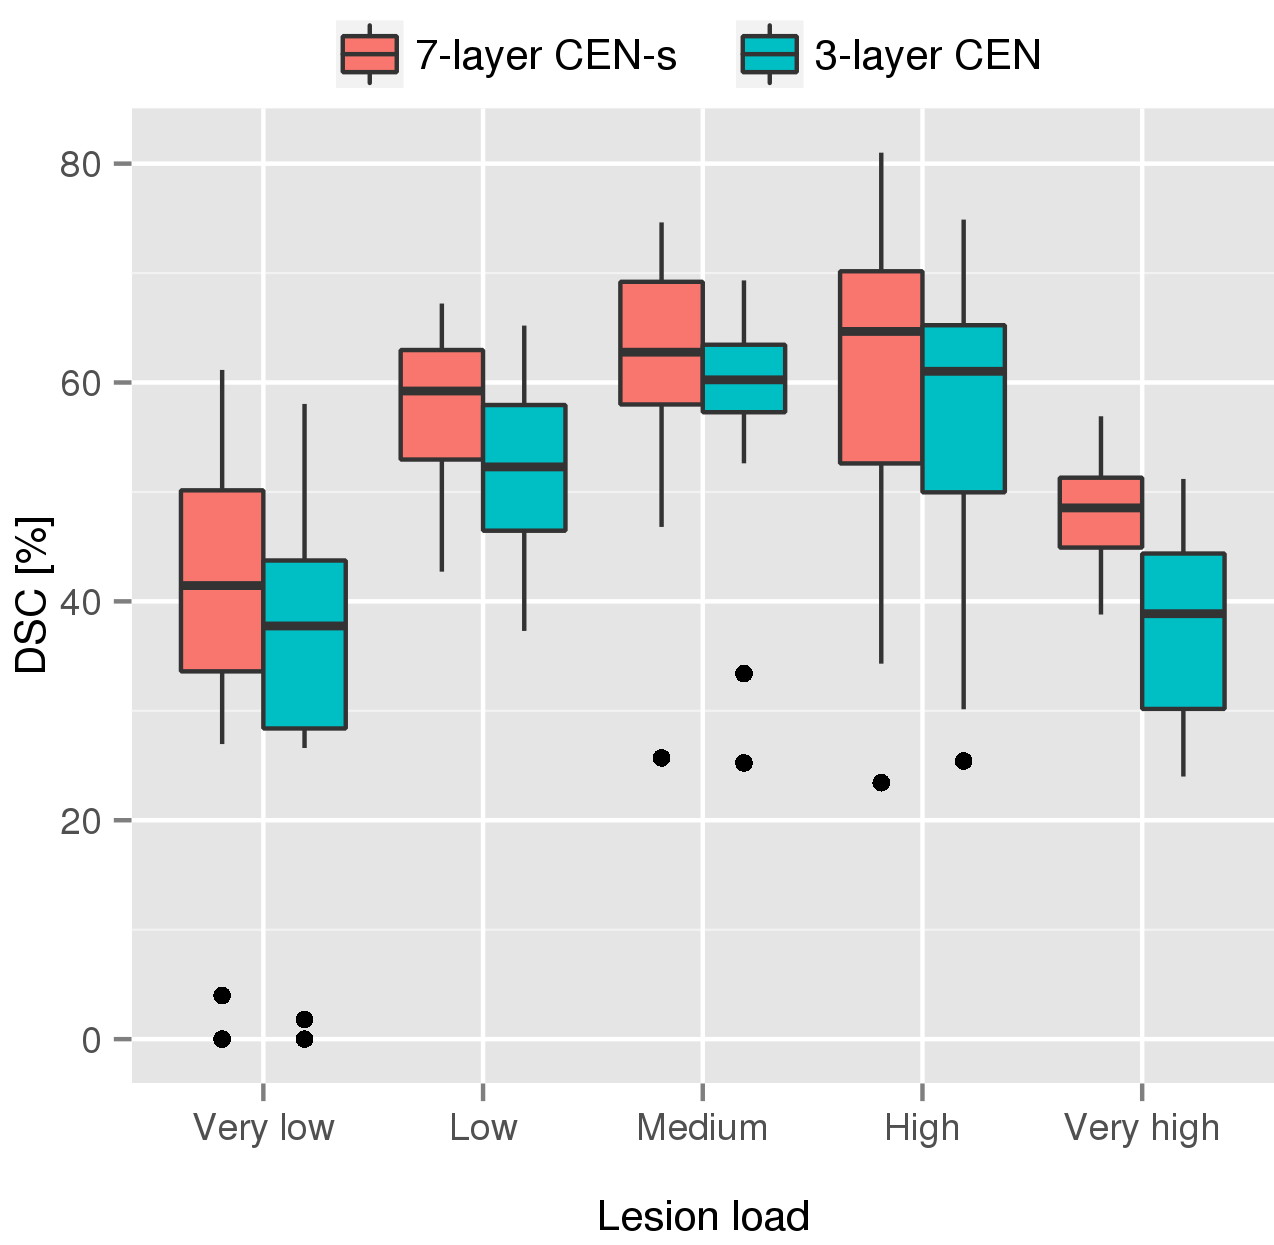
\includegraphics[width=\columnwidth]{figures/boxplot_L1vsL2}

\caption{Comparison of the segmentation accuracy measured by the DSC of a
3-layer CEN and a 7-layer CEN for different lesion load groups. Adding four layers and
shortcut connections improves the performance across all lesion loads, where the
improvements are especially large for scan with large lesion loads, which are
also correlated with an increase in lesion size.}

\label{fig:l1vl2}
\end{figure}

Fig.~\ref{fig:l2vlt} shows a comparison of the 7-layer CEN with shortcut
connections and Lesion-TOADS. The CEN approach performs more consistently
throughout all lesion load groups than Lesion-TOADS, where the improvements are
largest for very low to medium lesion loads. For very high lesion loads,
Lesion-TOADS achieves a higher mean DSC than the CEN approach. However, a
two-sided paired $t$-test yielded that the differences are not statistically
significant ($p\text{-value}=0.2566$). Table~\ref{tab:result2} shows a more
detailed comparison. While the PPV increases consistently with higher lesion
loads for both methods, the TPR is highest for low to medium lesion loads and
decreases again for high to very high lesion loads. This shows the difficulty
for both methods to correctly identify very large lesions that can extend far
into the white matter.

\begin{figure}[tb] \centering
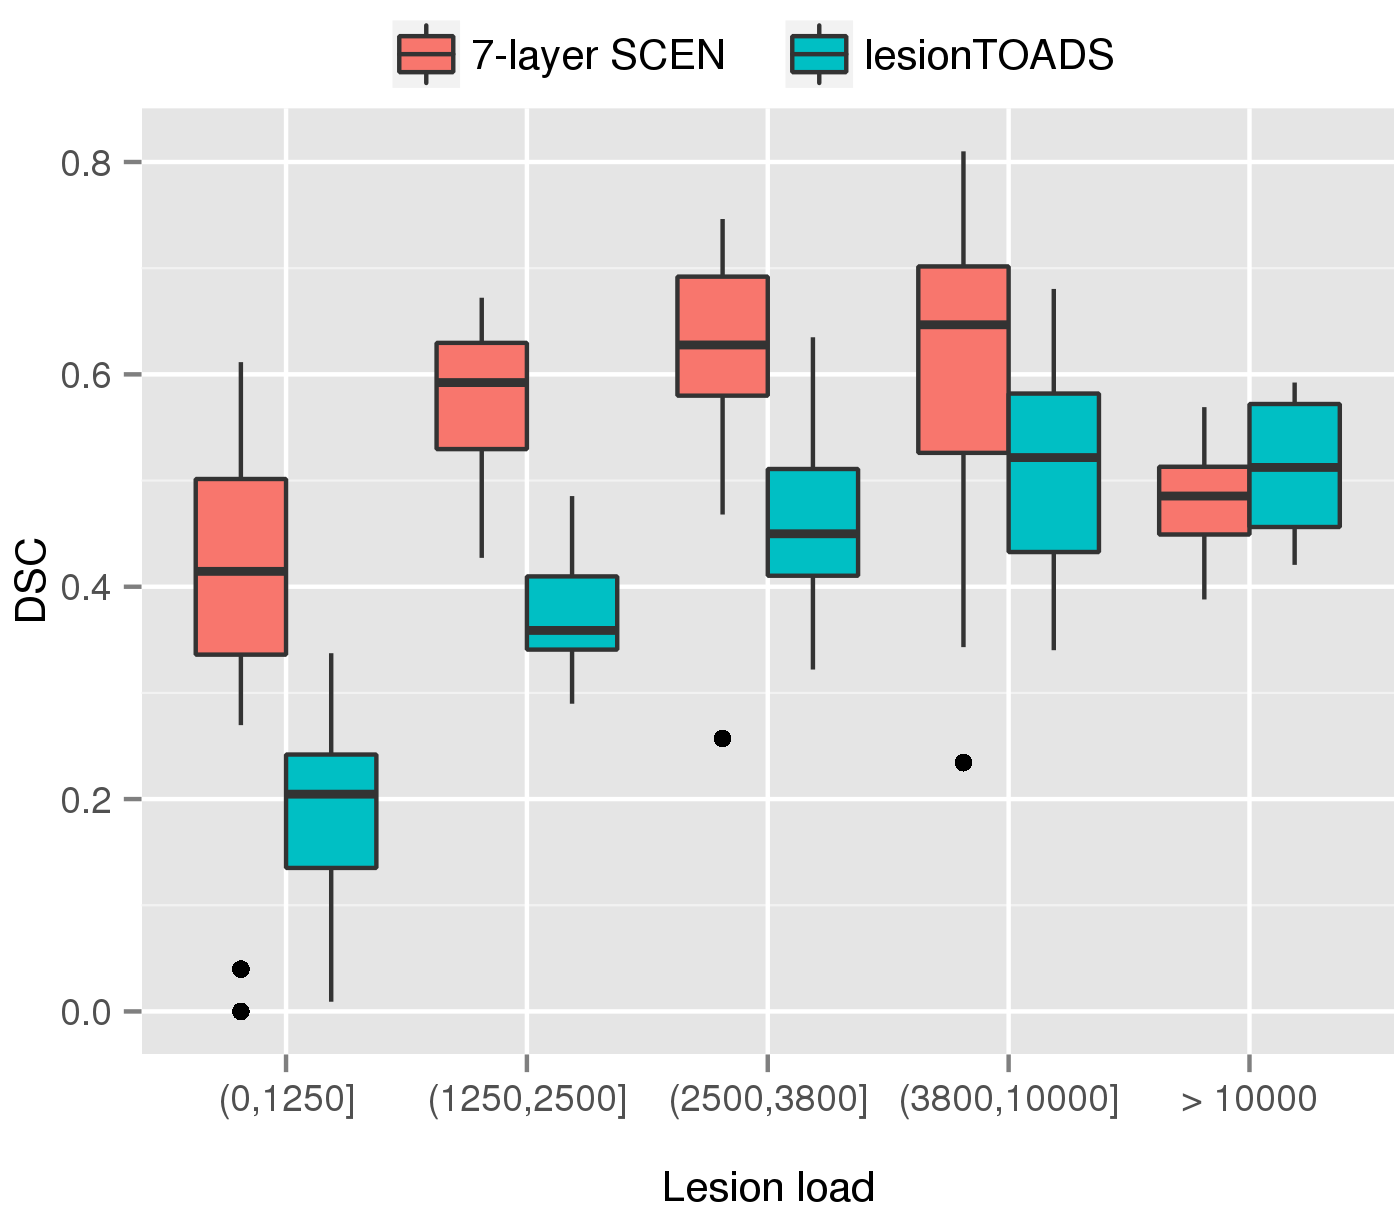
\includegraphics[width=\columnwidth]{figures/boxplot_L2vsLT}
\caption{Comparison of the segmentation accuracy measured by the DSC of
Lesion-TOADS and a 7-layer CEN with shortcut connections for different lesion
loads. The CEN approach is much more sensitive in detecting small lesions, while
still being able to detect large lesions.}
\label{fig:l2vlt}
\end{figure}

\begin{table}
\caption{Comparison of segmentation accuracy for different lesion load
categories.}
\label{tab:result2}
\begin{center}
\begin{tabular}{@{}ccccccc@{}}
\toprule
\multicolumn{1}{@{}l}{Lesion load} & \multicolumn{3}{c}{7-layer SCEN} &
\multicolumn{3}{c@{}}{Lesion-TOADS}
\\
& TPR & PPV & DSC & TPR & PPV & DSC \\
\midrule
\phantom{000}$(0,1250]$\phantom{0} & \num{50.00} & \num{41.15} & \num{39.34} &
\num{49.96} & \num{13.09} & \num{18.86}\\
$(1250,2500]$\phantom{0} & \num{61.92} & \num{59.01} & \num{57.45} & \num{52.39}
& \num{29.95} & \num{37.74}\\
$(2500,3800]$\phantom{0} & \num{57.64} & \num{71.54} & \num{61.31} & \num{54.17}
& \num{41.83} & \num{46.53}\\
$(3800,10000]$ & \num{51.14} & \num{81.11} & \num{60.13} & \num{47.97} &
\num{56.56} & \num{50.76}\\
$> 10000$ & \num{32.82} & \num{91.95} & \num{48.19} & \num{38.88} & \num{74.6} &
\num{50.93}\\
\bottomrule
\end{tabular}
\end{center}
\end{table}

% \begin{itemize}
% \item Have some sample images and discuss what we can see here.
% \end{itemize}

\subsection{Qualitative Results}

A qualitative comparison of segmentation performance for four characteristic
cases is shown in Fig.~\ref{fig:images}. Our method produces segmentations that
are spatially consistent (see Fig.~\ref{fig:images}a), while still being able to
detect small isolated lesions (green circle). Furthermore, our method is able to
learn a wide spectrum of lesion shapes and appearances from training data. This
allows our method to correctly identify multiple different types of MS lesions
(e.g., T1 black holes), which can be challenging to detect for Lesion-TOADS (see
Fig.~\ref{fig:images}b).
Our method uses a combination of automatically learned intensity and appearance
features, which makes it inherently robust to noise as shown in
Fig.~\ref{fig:images}c. Figure~\ref{fig:images}d shows one of the most
challenging cases for our method. Very large lesions might extend beyond the
size of the receptive field of the CEN, which reduces its ability to extract
characteristic lesion features. Consequently, our method might underestimate
the size of very large lesions for some cases.

\begin{figure*}
%\centering
\hspace*{-5pt}
\subfloat[Spatially consistent segmentation] {
\begin{tikzpicture}[node distance=1.5cm and 0.2\columnwidth,
  font=\footnotesize, on grid]
  
\node[,inner sep=0] (image) {
  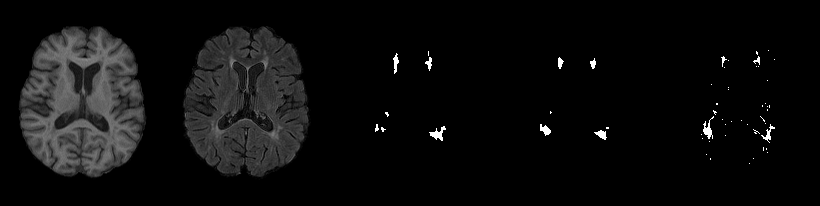
\includegraphics[width=\columnwidth]{figures/p17s29_noisy_lesionTOADS} };
\node[above=of image] (gt) {\phantom{g}Ground truth\phantom{g}};
\node[left=of gt] (flair) {\phantom{g}FLAIR\phantom{g}};
\node[left=of flair] {T1-weighted};
\node[right=of gt,align=center] (cen) {\phantom{g}Our method\phantom{g}};
\node[right=of cen,align=center] {Lesion-\\ TOADS};

\draw[green, thick] (-7pt,-3.5pt) circle (3pt);
\begin{scope}[xshift=0.2\columnwidth]
\draw[green, thick] (-7pt,-3.5pt) circle (3pt);
\end{scope}

\end{tikzpicture}
}
\subfloat[Can handle multiple types of lesions (e.g., T1 black holes)
correctly] {
\begin{tikzpicture}[node distance=1.5cm and 0.2\columnwidth,
  font=\footnotesize, on grid]
  
\node[,inner sep=0] (image) {
  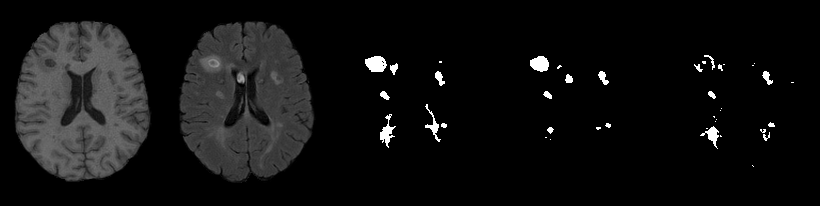
\includegraphics[width=\columnwidth]{figures/p36s30_blackhole}};
\node[above=of image] (gt) {\phantom{g}Ground truth\phantom{g}};
\node[left=of gt] (flair) {\phantom{g}FLAIR\phantom{g}};
\node[left=of flair] {T1-weighted};
\node[right=of gt,align=center] (cen) {\phantom{g}Our method\phantom{g}};
\node[right=of cen,align=center] {Lesion-\\ TOADS};

\draw[red,thick] (-10pt,12pt) circle (7pt);
\begin{scope}[xshift=-0.2\columnwidth]
\draw[red,thick] (-10pt,12pt) circle (7pt);
\end{scope}
\begin{scope}[xshift=-0.4\columnwidth]
\draw[red,thick] (-10pt,12pt) circle (7pt);
\end{scope}
\begin{scope}[xshift=0.2\columnwidth]
\draw[red,thick] (-10pt,12pt) circle (7pt);
\end{scope}
\begin{scope}[xshift=0.4\columnwidth]
\draw[red,thick] (-10pt,12pt) circle (7pt);
\end{scope}

\end{tikzpicture}
}\\
\hspace*{-5pt}
\subfloat[Robust to noise] {
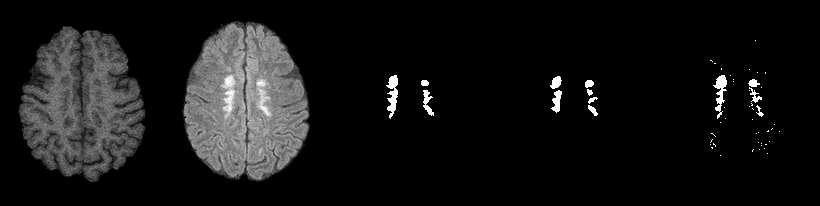
\includegraphics[width=\columnwidth]{figures/p15s34_robust_to_noise3}
}
\subfloat[Underestimates very large lesions] {
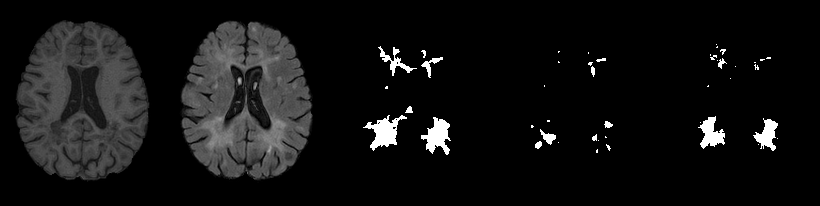
\includegraphics[width=\columnwidth]{figures/p54s32_large_lesions}
}

\caption{Four cases illustrating the strengths and weaknesses of our method
compared to Lesion-TOADS. Our method is able a) to produce spatially consistent
segmentations, b) to handle multiple different types of lesions correctly (e.g.,
T1 black holes), and c) is inherently robust to noise. (d) Our method
might underestimate the size of very large lesions for some cases.}

\label{fig:images}
\end{figure*}

\begin{comment}
\subsection{BioMS Data Set}

\begin{table}
\caption{Training results on the BioMS data set using 150 and 250 images for
training.}
\begin{center}
\begin{tabular}{llcc}
\toprule
Pre-training & Fine-tuning & Training DSC & Test DSC \\
\midrule
With dropout & Hessian-free (150) & 67.1 & 61.7 \\
With dropout & Hessian-free (250) & 68.0 & 62.8 \\
Without dropout & Hessian-free (150) & 66.5 & 61.7 \\
With dropout & AdaDelta (150) & 65.9 & 60.6 \\
Without dropout & AdaDelta (150) & 66.0 & 60.6 \\
\bottomrule
\end{tabular}
\end{center}
Notes: No comparison with
state-of-the-art methods are available here. The effect of dropout in the
pre-training phase on the final result is negligible. Hessian-free is slightly
better than AdaDelta and does not require the tuning of parameters. However,
Hessian-free optimization does not support dropout, which might be important
for regularization when the data set size is small or the number of layers and
filters is high.
\end{table}
\end{comment}

% \subsection{On a small data set}
% 
% Include MICCAI challenge results, because it was a comparison with more methods.

\begin{comment}
\subsection{Evaluation of Training Methods}

We have evaluated the impact of different training and initialization methods on
the performance of the trained network using the example of a 7-layer CEN. The
network architecture is summarized in Table~\ref{tab:arch7}. All methods have
hyperparameters, which can be difficult to choose. To find a good set of
hyperparameters for each algorithm (except for Hessian-free), we first trained
the model for 20 epochs with the hyperparameters shown in
Table~\ref{tab:parameters}. We then used the set of parameters that produced the
lowest error on the training set to further fine-tune the model for 500 epochs.
This tuning procedure favors algorithms that are robust to the choice of the
hyperparameters or can make substantial progress within the first few epochs,
which are both desirable properties of a training method for which
time-consuming parameter tuning using a large number of epochs and
cross-validation is not feasible. As is the case for the training on large data
sets on high-resolution 3D medical images. The hyperparameters of the
Hessian-free optimization are very robust to the choice of input data. We found
that tuning these parameters is not necessary. Another difference of the
Hessian-free optimization compared to the other methods is that HF is able to
make more progress within an epoch, albeit at the cost of more time-consuming
updates. To compensate, we trained HF for only 22 epochs. Parameter estimation
and fine-tuning of the model required 2.9 GB of GPU memory and took
approximately 42 hours on a single NVIDIA GeForce GTX 780 graphics card.
However, once the model has been trained, segmentation of an entire 3D image can
be performed in less than half a seconds.

\begin{table}
\caption{Algorithm parameters}%
\label{tab:parameters}
\begin{center}
\begin{tabular}{@{}lp{0.7\columnwidth}@{}}
\toprule
Algorithm & Parameters \\
\midrule
SGD \cite{LeCun1998} & $\text{learning rate} \in \{\num{e-3}, \num{e-4}, \num{e-5},
\num{e-6}\},\newline \text{momentum} = 0.9$ \\

AdaGrad \cite{duchi2011adaptive} & $\alpha \in \{\num{e-4}, \num{e-5},
\num{e-6}, \num{e-7}\}, \epsilon = \num{e-11}$ \\

Adam \cite{kingma2014adam} & $\alpha \in \{\num{3e-5}, \num{e-5}, \num{e-6},
\num{e-7}\}$, $\beta_1 = 0.1$, \newline $\beta_2 = 0.001$, $\epsilon = \num{e-11}$ \\

AdaDelta \cite{zeiler2012adadelta} & $\epsilon \in \{\num{e-9}, \num{e-10},
\num{e-11}\}, \rho= 0.95$
\\

RMSProp \cite{dauphin2015rmsprop} & $\epsilon \in \{\num{e-4}, \num{e-5},
\num{e-6}, \num{e-7}\}, \alpha = 0.9 $\\

Hessian-free \cite{martens2010deep} & $\lambda_0 = 1, \zeta = 0.9$ \\
\bottomrule
\end{tabular}
\end{center}
Note: Please refer to the respective paper for a detailed description of the
hyperparameters.
\end{table}

Figure~\ref{fig:methods} shows a comparison of Dice similarity coefficients
calculated on the test set after training the 7-layer CEN with different
optimization methods as well as with and without pre-training. The results for
SGD are not included in the figure, because we were not able to find a learning
rate for which SGD can make notable progress.
\begin{itemize}
\item SGD is not included because the training method failed to make notable
progress
\item A possible explanation is that the parameters of different layers vary
greatly in magnitude and therefore require different learning rates
\item However, SGD used the same learning rate for all layers and the tuning
phase was not able to find a learning rate that works for all layers
\item In addition, none of the first-order methods were able to train the
CEN without pre-training, which further highlights the difficulty of training deep
CNNs on sparse segmentations.
\item We found that pre-training is crucial to alleviate the difficulty of
training deep CNNs with very unbalanced classes.
\item The training algorithms AdaDelta, Adam, Hessian-free and RMSProp perform
roughly the same with only AdaGrad notably worse than the other methods.
\item Hessian-free optimization was the only method that did not require
pre-training, where the results with pre-training are still slightly better than
without pre-training
\end{itemize}  

\begin{figure}[tb]
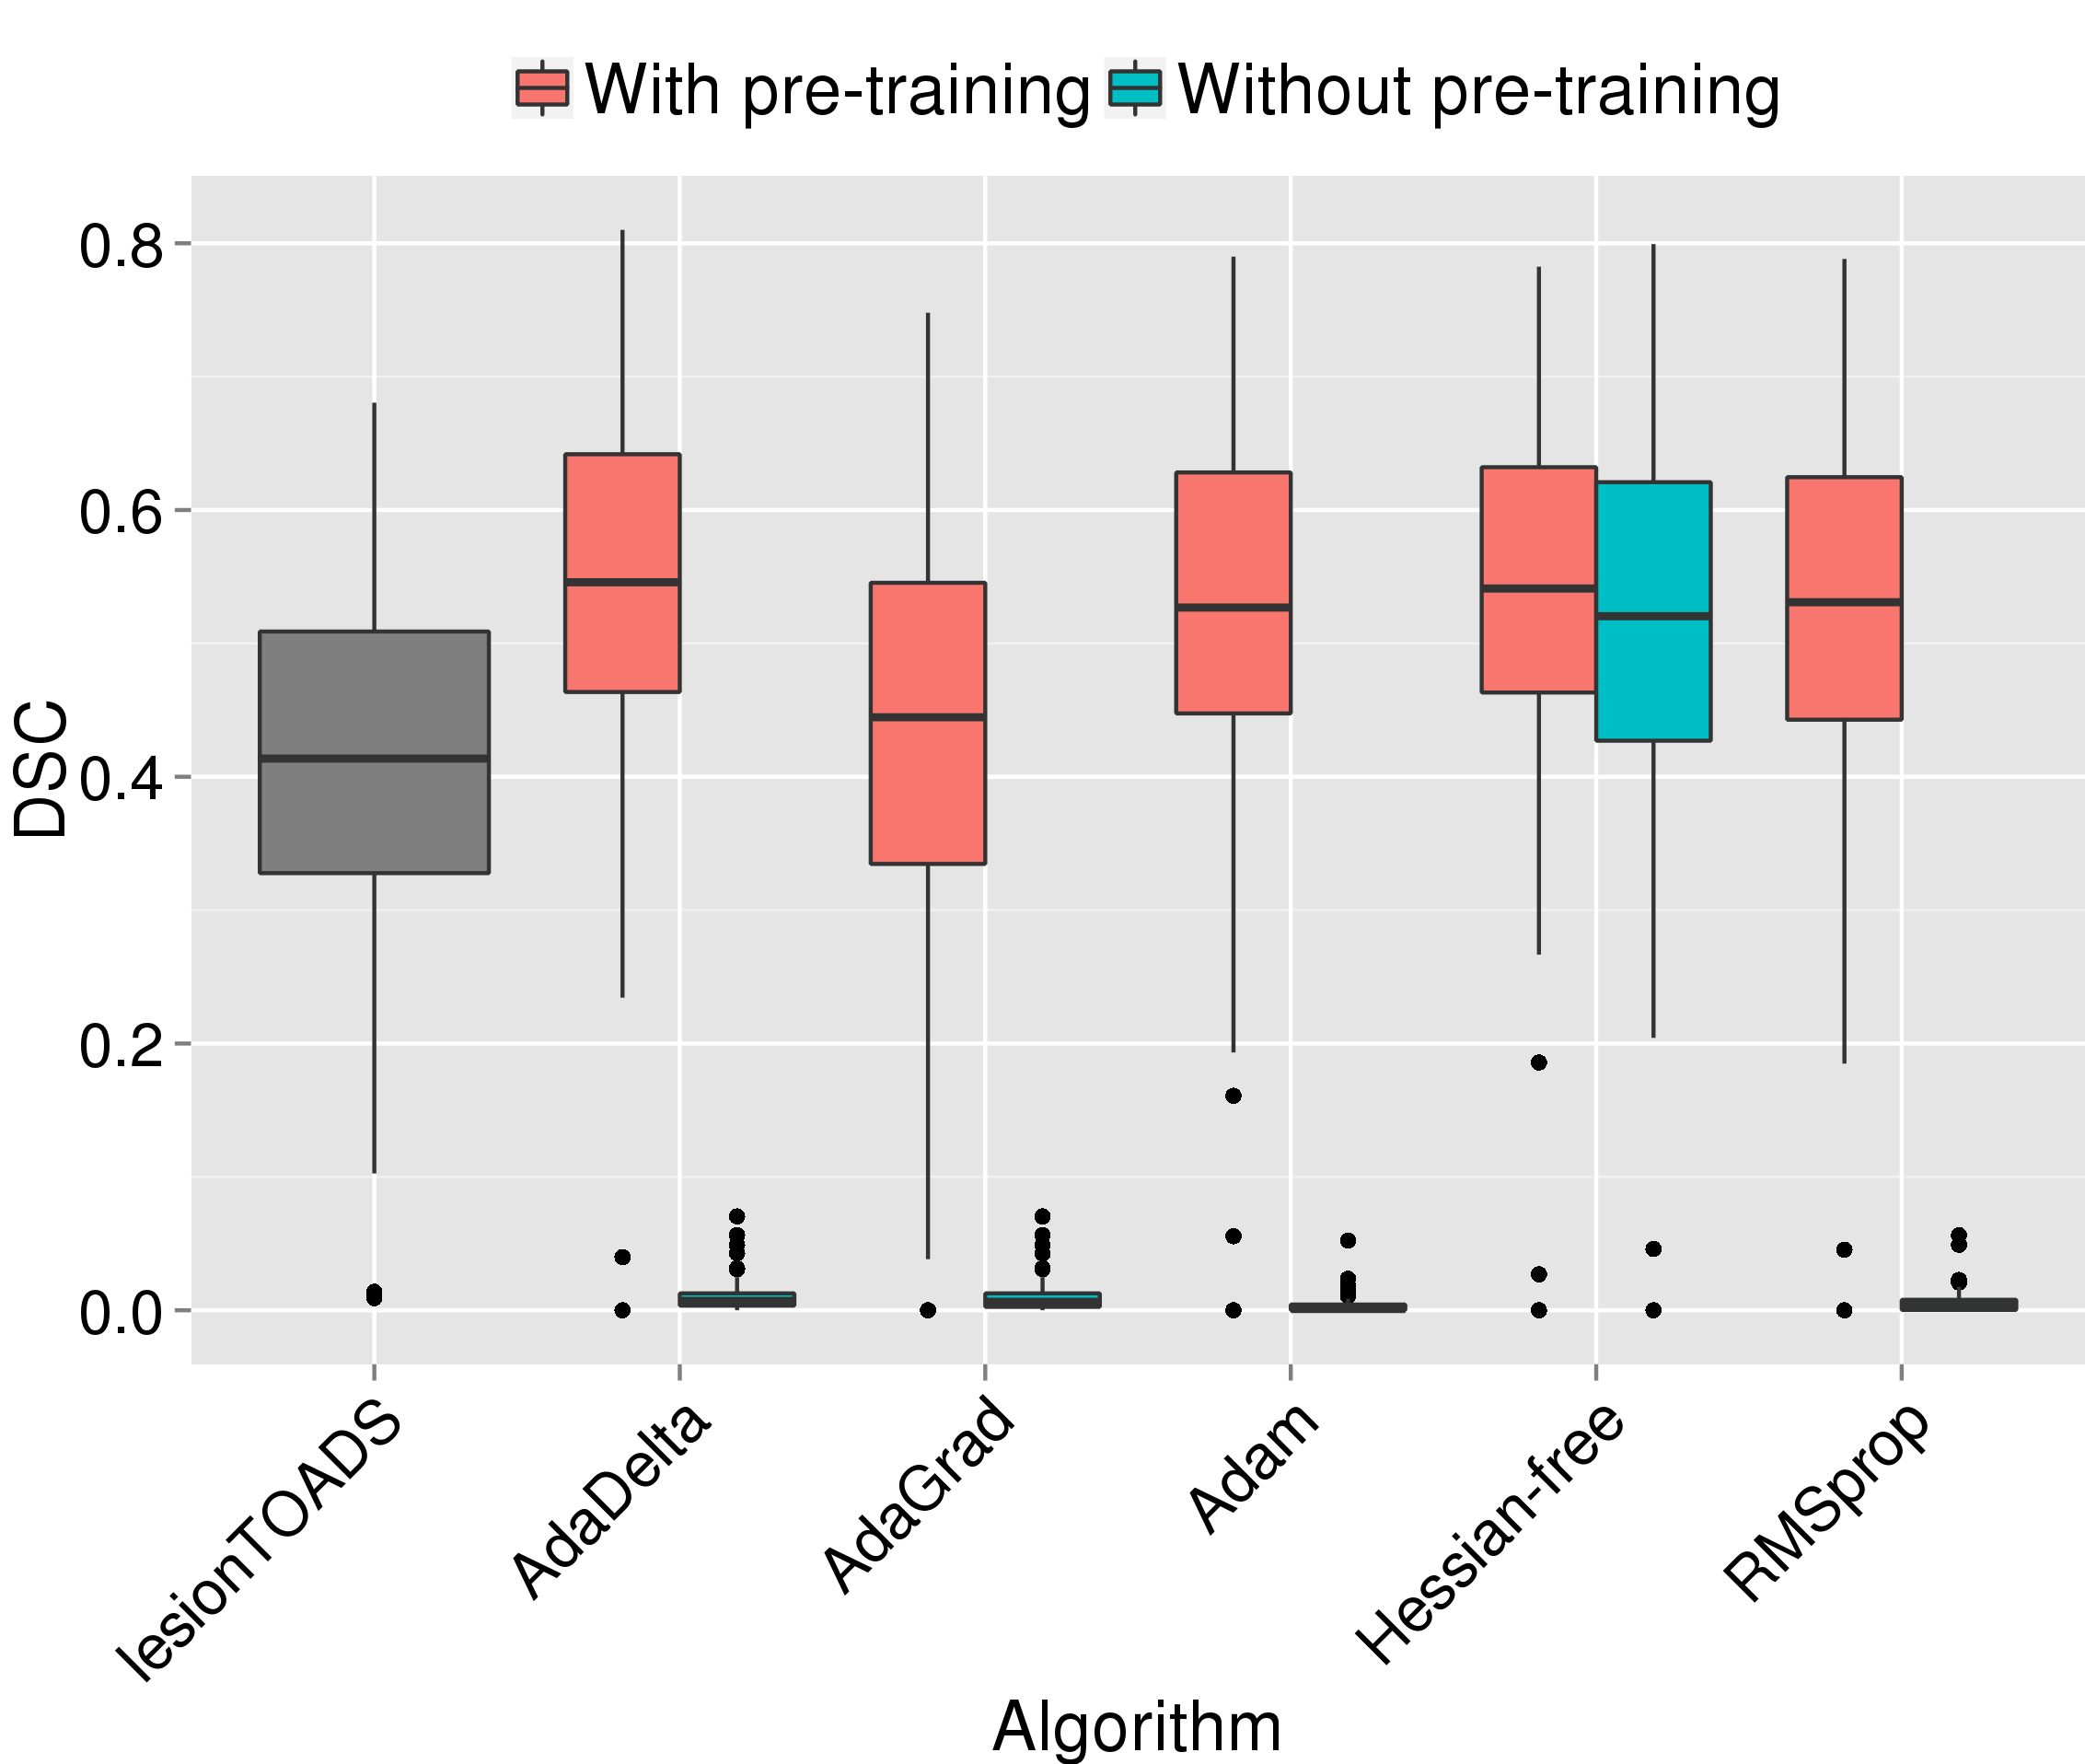
\includegraphics[width=\columnwidth]{figures/methods2}
\caption{Comparison of different training methods with pre-training (left) and
without pre-training (right). Hessian-free is the only method that does not
require pre-training to train the model. With pre-training, AdaDelta, Adam,
Hessian-free, and RMSprop consistently learn models that perform significantly
better than lesionTOADS.}
\label{fig:methods}
\end{figure}

A more detailed comparison of the 7-layer CEN trained with different
optimization algorithms and lesionTOADS is summarized in Table~\ref{tab:results1}.
\begin{itemize}
\item TPR is comparable to lesionTOADS, whereby only the CEN trained with
AdaDelta is able to achieve a higher TPR than lesionTOADS
\item Advantage of CEN model is the much reduces number of false positives,
which results in a significantly higher PPV.
\item All methods, except for AdaGrad, outperform lesionTOADS in terms of the
DCS by more than \SI{10}{\percent}. The best performing method achieves a DSC of
\num{54.02} compared to a DSC of \num{40.04} achieved by lesionTOADS on this
challenging data set.
\end{itemize}

\begin{table}
\sisetup{separate-uncertainty=true,detect-weight=true,detect-inline-weight=math}
\begin{center}
\caption{Comparison of the segmentation accuracy of a 7-layer CEN trained with
different algorithms and lesionTOADS}
\label{tab:results1}
\begin{tabular}{@{}lccc@{}}
\toprule
Algorithm & TPR [\%] & PPV [\%] & DSC [\%] \\
\midrule
AdaDelta & \textbf{\num{52.75+-20.31}} & \num{66.58+-20.71} &
\textbf{\num{54.02+-15.24}} \\
AdaGrad & \num{42.14+-18.88} & \num{54.65+-20.24} & \num{43.21+-15.05} \\
Adam & \num{47.41+-18.96} & \textbf{\num{70.33+-20.98}} & \num{51.93+-15.08} \\
Hessian-free & \num{49.21+-18.76} & \num{68.33+-21.12} & \num{52.65+-15.09} \\
RMSprop & \num{47.9+-20.53} & \num{69.12+-20.78} & \num{51.46+-15.77} \\[0.4em]
lesionTOADS & \num{49.83+-14.79} & \num{39.86+-20.95} & \num{40.04+-14.86} \\
\bottomrule
\end{tabular}
\end{center}
Note: The table shows the mean and standard deviation of the true positive rate
(TPR), positive predictive value (PPV), and Dice similarity coefficient (DSC).
All experiments were performed with pre-training and evaluated on the test set.
\end{table}

\subsection{Evaluation of Network Architectures}

In a second experiment, we evaluated the impact of the network architecture on
the segmentation performance. Therefore, we have trained different networks with
varying number of layers and with and without shortcut connections between the
convolutional and deconvolutional pathway. Table~\ref{tab:arch15} shows the
parameters of a 15-layer CEN. We have used the same parameters for the 11-layer,
7-layer, and 3-layer CENs with the respective layers removed.
\begin{itemize}
\item Shortcut connections are increasingly more important with increasing
depth of the network
\item The DSC decreases with depth without shortcut while it increases with
shortcuts
\item After 11 layers, the network performance does not increase on the test set
as the network starts to overfit more
\item Either more training data or better regularization methods are needed to
train very deep models
\end{itemize}

\begin{table}[tb]
\caption{Parameters of the 15 layers of the CENs used to evaluate different
network architectures.}
\label{tab:arch15}
\begin{center}
\begin{tabular}{@{}lccr@{}}
\toprule
Layer type & Kernel size & Filters & \multicolumn{1}{c}{Image size} \\
\midrule
Input & --- & --- & \num{164x206x52x2}\phantom{0} \\
Convolutional & \num{9x9x5x2} & 32 & \num{156x198x48x32} \\
Average Pooling & \num{2x2x2} & --- & \num{78x99x24x32} \\
Convolutional & \num{9x10x5x32} & 32 & \num{70x90x20x32} \\
Average Pooling & \num{2x2x1} & --- & \num{35x45x20x32} \\
Convolutional & \num{8x10x5x32}  & 32 & \num{28x36x16x32} \\
Average Pooling & \num{2x2x1} & --- & \num{14x18x16x32} \\
Convolutional & \num{7x11x9x32}  & 32 & \num{8x8x8x32} \\
Deconvolutional & \num{7x11x9x32}  & 32 & \num{14x18x16x32} \\
Unpooling & \num{2x2x1}       & --- & \num{28x36x16x32} \\
Deconvolutional & \num{8x10x5x32} & 32 & \num{35x45x20x32} \\
Unpooling & \num{2x2x1}       & --- & \num{70x90x20x32} \\  
Deconvolutional & \num{9x10x5x32} & 32 & \num{78x99x24x32} \\
Unpooling & \num{2x2x2} & --- & \num{156x198x48x32} \\
Deconvolutional & \num{9x9x5x32} & 1 & \num{164x206x52x1}\phantom{0} \\
\bottomrule
\end{tabular}
\end{center}
Note: Networks with fewer layer use the same parameters as the 15-layer
CEN, where the missing layers are simply removed.
\end{table}

Analysis of different training set sizes
\begin{itemize}
\item Varying number of training samples
\item With dropout and without (regularization)
\item Performed on most promising architecture
\item Possible outcome: to harsh regularization decreases performance when
enough training data is available but improves performance for small data sets
due to the reduction of overfitting
\end{itemize}
\end{comment}

% \begin{table}
% \caption{Preliminary segmentation results on the Bravo data set.}
% \begin{center}
% \begin{tabular}{lc}
% \toprule
% Method & Training and test DSCs \\
% \midrule
% Input pre-training, 1-layer CNN &  41.63 / 42.76 \\[0.25em]
% No pre-training, 2-layer CNN & 51.88 / 46.93 \\
% Joint pre-training, 2-layer CNN & 44.52 / 43.82 \\
% Input pre-training, 2-layer CNN & 51.02 / 46.58 \\[0.25em]
% Input pre-training, 4-layer CNN & 59.60 / 46.14 \\[0.25em]
% Lesion-TOADS & \phantom{00.}--- / 34.87 \\
% \bottomrule
% \end{tabular}
% \end{center}
% Note: All tests were performed with Hessian-free optimization. Pre-training was
% always performed with dropout.
% \end{table}

\begin{comment}


To allow for a direct comparison with state-of-the-art lesion segmentation
methods, we evaluated our method on the FLAIR, T1-, and T2-weighted MRIs of the
20 publicly available labeled cases from the MS lesion segmentation challenge
2008 \cite{styner20083d}, which we downsampled from the original isotropic voxel
size of \SI{0.5}{\cubic\milli\metre} to an isotropic voxel size of
\SI{1.0}{\cubic\milli\metre}. In addition, we evaluated our method on an
in-house data set from an MS clinical trial of 500 subjects split equally into
training and test sets. The images were acquired from 45 different scanning
sites. For each subject, the data set contains T2- and PD-weighted MRIs with a
voxel size of \SI{0.937x0.937x3.000}{\milli\metre}. The main preprocessing steps
included rigid intra-subject registration, brain extraction, intensity
normalization, and background cropping.

We used a CEN with 32 filters and filter sizes of \num{9x9x9} and \num{9x9x5}
voxels for the challenge and in-house data sets, respectively. Training on a
single GeForce GTX 780 graphics card took between 6 and 32 hours per model
depending on the training set size. However, once the network is trained,
segmentation of trimodal 3D volumes with a resolution of, e.g.,
\num{159x201x155} voxels can be performed in less than one second. As a
rough\footnote{Ciresan et al. used a more complex network that is composed of 11
layers. However, their network was trained on much smaller images, which roughly
compensates for the increased complexity.} comparison, Ciresan et al.
\cite{Ciresan2012} reported that their patch-based method required 10 to 30
minutes to segment a single 2D image with a resolution of \num{512x512} voxels
using four graphics cards, which demonstrates the large speed-ups gained by
processing entire volumes.

% \begin{figure}[tb]
% \centering
% \small
% \def\MRIwidth{0.15\textwidth}
% 
% \begin{tikzpicture} 
% \tikzstyle{leftlabel}=[rotate=90, align=center,overlay,above]
% 
% \matrix [matrix of nodes, nodes={anchor=center, inner sep=1pt}] {
%         &[4pt] FLAIR & T1w & T2w & Ground truth & Our method \\[4pt]
% \node[leftlabel] {CHB\,07\\(DSC\,=\,\SI{60.58}{\percent})}; &
% 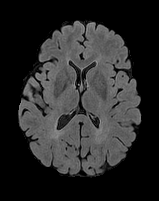
\includegraphics[width=\MRIwidth]{figures/CHB07-FLAIR-s88} &
% 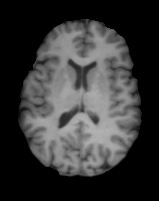
\includegraphics[width=\MRIwidth]{figures/CHB07-T1w-s88} &
% 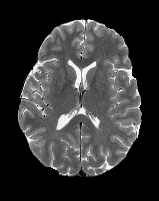
\includegraphics[width=\MRIwidth]{figures/CHB07-T2w-s88} &
% 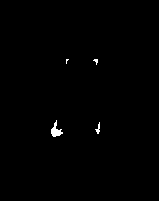
\includegraphics[width=\MRIwidth]{figures/CHB07-gold-s88} &
% 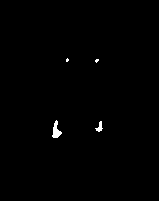
\includegraphics[width=\MRIwidth]{figures/CHB07-pred-s88} \\
% \node[leftlabel] {CHB\,04\\(DSC\,=\,\SI{61.37}{\percent})}; &
% 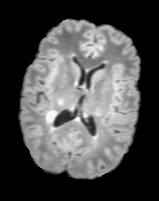
\includegraphics[width=\MRIwidth]{figures/CHB04-FLAIR-s85} &
% 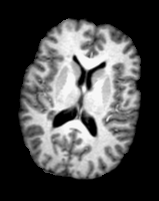
\includegraphics[width=\MRIwidth]{figures/CHB04-T1w-s85} &
% 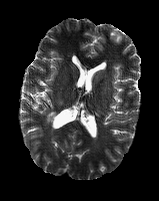
\includegraphics[width=\MRIwidth]{figures/CHB04-T2w-s85} &
% 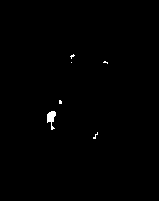
\includegraphics[width=\MRIwidth]{figures/CHB04-gold-s85} &
% 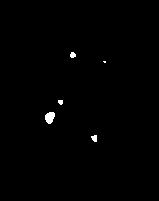
\includegraphics[width=\MRIwidth]{figures/CHB04-pred-s85} \\
% \node[leftlabel] {UNC\,09\\(DSC\,=\,\SI{9.01}{\percent})}; &
% 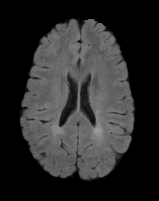
\includegraphics[width=\MRIwidth]{figures/UNC09-FLAIR-s89} &
% 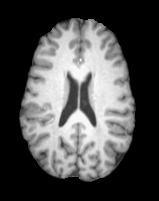
\includegraphics[width=\MRIwidth]{figures/UNC09-T1w-s89} &
% 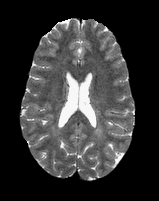
\includegraphics[width=\MRIwidth]{figures/UNC09-T2w-s89} &
% 
\includegraphics[width=\MRIwidth]{figures/UNC09-gold-s89} &
% 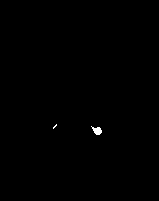
\includegraphics[width=\MRIwidth]{figures/UNC09-pred-s89} \\
% };
% \end{tikzpicture}
% 
% \caption{Example segmentations of our method for three different subjects from
% the challenge data set. Our method performed well and consistently despite the
% large contrast differences seen between the first two rows. In the third row,
% our method also segmented lesions that have similar contrast, but these regions
% had not been identified as lesions by the manual rater, which highlights the
% difficulty in distinguishing focal lesions from diffuse damage, even for
% experts.}
% 
% \label{fig:segmentation}
% \end{figure}

We evaluated our method on the challenge data set using 5-fold
cross-valida\-tion and calculated the true positive rate (TPR), positive
predictive value (PPV), and Dice similarity coefficient (DSC) between the
predicted segmentations and the resampled ground truth.
Figure~\ref{fig:segmentation} shows a comparison of three subjects from the
challenge data set. The first two rows show the FLAIR, T1w, T2w, ground truth
segmentations, and predicted segmentations of two subjects with a DSC of
\SI{60.58}{\percent} and \SI{61.37}{\percent}. Despite the large contrast
differences between the two subjects, our method performed well and
consistently, which indicates that our model was able to learn features that are
robust to a large range of intensity variations. The last row shows a subject
with a DSC of \SI{9.01}{\percent}, one of the lowest DSC scores from the data
set. Our method segmented lesions that have similar contrast to the other two
subjects, but these regions were not classified as lesions by the manual rater.
This highlights the difficulty of manual lesion segmentation, as the difference
between diffuse white matter pathology and focal lesions is often indistinct. A
quantitative comparison of our method with other state-of-the-art methods is
summarized in Table~\ref{tab:state}. Our method outperforms the winning method
(Souplet et al. \cite{souplet2008}) of the MS lesion segmentation challenge 2008
and the currently best unsupervised method reported on that data set (Weiss et
al. \cite{weiss2013}) in terms of mean TPR and PPV. Our method performs
comparably to a current method (Geremia et al. \cite{geremia2010}) that uses a
carefully designed set of features specifically designed for lesion
segmentation, despite our method having learned its features solely from a
relatively small training set.

\begin{table}[tb]
\def\tabspace{12pt}

\caption{Comparison of our method with state-of-the-art lesion segmentation
methods in terms of mean TPR, PPV, and DSC. Our method performs comparably to
the best methods reported on the MS lesion segmentation challenge data set.}

\label{tab:state}
\centering
\begin{tabular}{l%
@{\hspace{\tabspace}}S[table-format=2.2]
@{\hspace{\tabspace}}S[table-format=2.2]
@{\hspace{\tabspace}}S[table-format=2.2]
}
\toprule
Method & {TPR} & {PPV} & {DSC} \\ 
\midrule
Souplet et al. \cite{souplet2008} & 20.65 & 30.00 & {---} \\ 
Weiss et al. \cite{weiss2013} & 33.00 & 36.85 & 29.05 \\ 
Geremia et al. \cite{geremia2010} & 39.85 & 40.35 & {---}  \\
Our method & 39.71 & 41.38 & 35.52 \\
\bottomrule
\end{tabular}
\end{table}

To evaluate the impact of the training set size on the segmentation performance,
we trained our model on our in-house data set with a varying number of training
samples and calculated the mean DSC on the training and test sets as illustrated
in Fig.~\ref{fig:bioms}. For small training sets, there is a large difference
between the DSCs on the training and test sets, which indicates that the
training set is too small to learn a representative set of features. At around
100 samples, the model becomes stable in terms of test performance and the small
difference between training and test DSCs, indicating that overfitting of the
training data is no longer occurring. With 100 training subjects, our method
achieves a mean DSC on the test set of \SI{57.38}{\percent}, which shows that
the segmentation accuracy can be greatly improved compared to the results on the
challenge data set, when a representative training set is available.

\begin{figure}[tb]
\centering
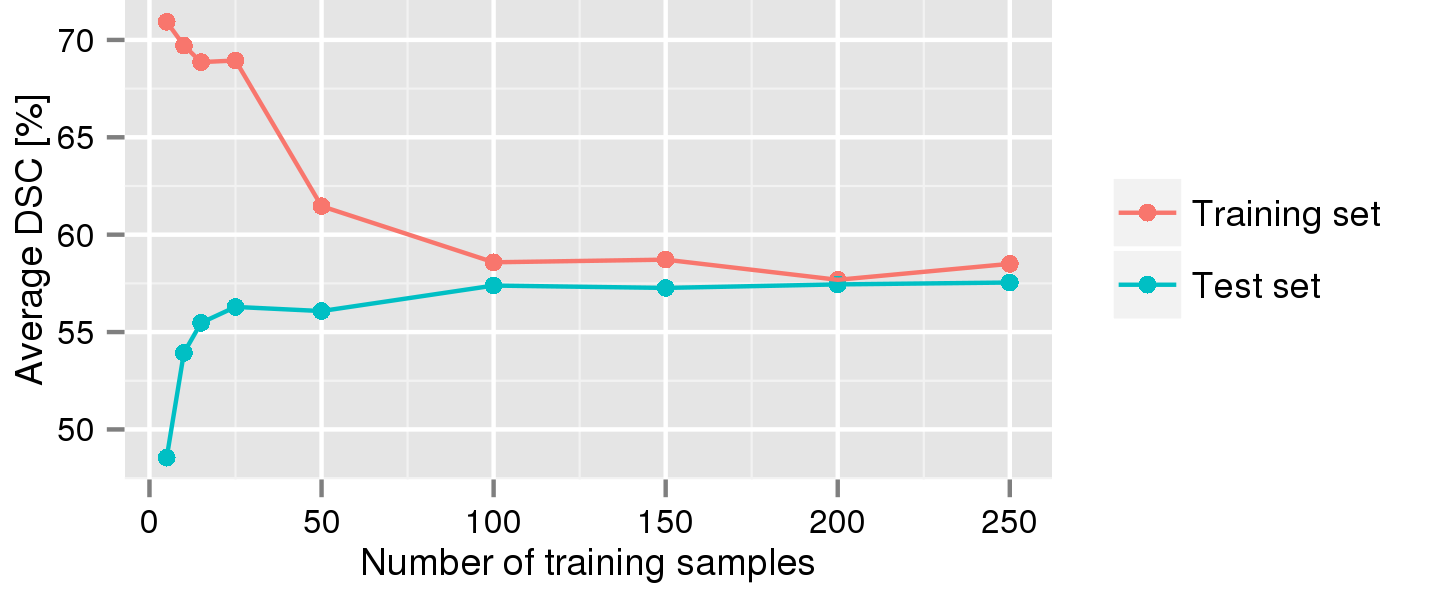
\includegraphics[width=0.78\textwidth]{figures/train_count}

\caption{Comparison of DSC scores calculated on the training and test sets for
varying numbers of training samples. At around 100 samples, the model becomes
stable in terms of test performance and the small difference between training
and test DSCs, indicating that overfitting of the training data no longer
occurs.}
\label{fig:bioms}
\end{figure}

\end{comment}
